\chapter{Convolutional Neural Networks}\label{ch:cnn}
Convolutional Neural Networks (CNNs) are a group of models which allow for efficient training on high dimensional data.
This is especially useful in the field of computer vision as image data is fundamentally high dimensional.
This feat was achieved by application of two principles: \textit{invariance}~\ref{subsec:invariance} and
\textit{locality}~\ref{subsec:locality}

\begin{figure}[H]
    \centering
    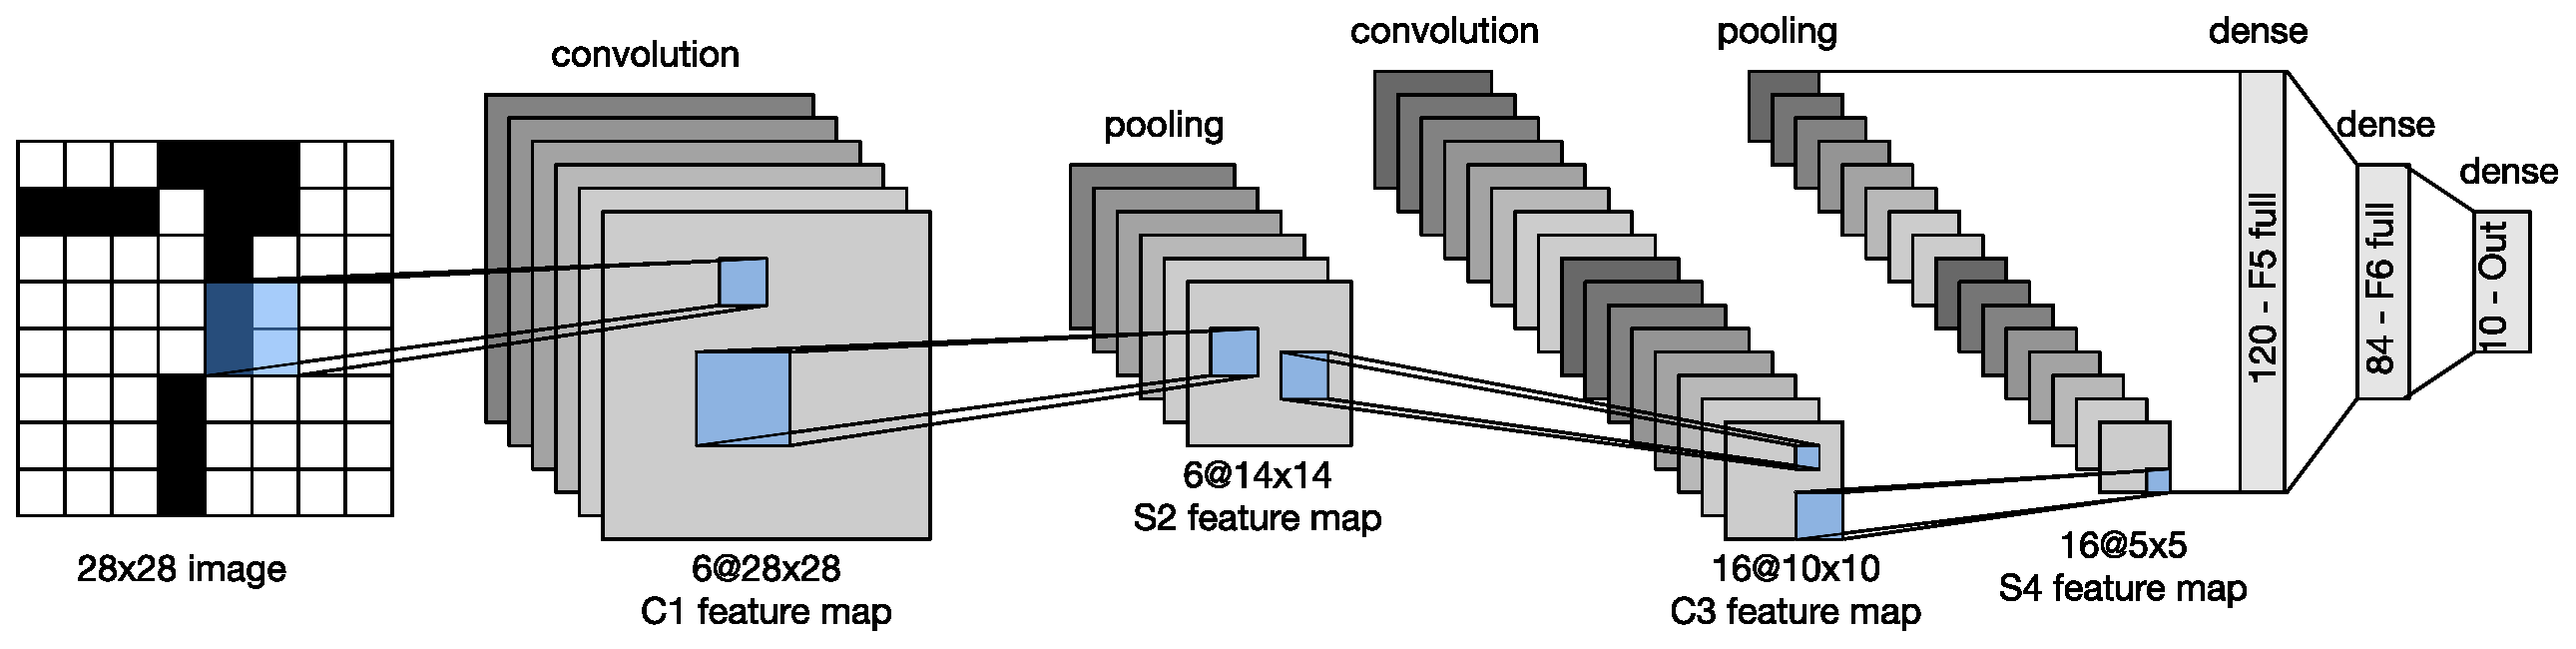
\includegraphics[width=\columnwidth]{images/cnn/lenet.eps}
    \caption{Example of CNN model (LeNet 5)~\cite{CNN}}
    \label{fig:cnn}
\end{figure}

As we can see in the illustration~\ref{fig:cnn} the model contains many layers.
This is typical for CNNs and it's a reason why CNNs belong to the class of machine learning methods called
\textit{deep learning}\footnote{Set of machine learning models with
\textit{credit assignment path (CAP)} higher than 2.
The CAP is the chain of transformations from input to output.}
Typically there are three layer types stacked in the CNN model: \textit{dense}~\ref{sec:dense},
\textit{convolutional}~\ref{sec:convolutional} and \textit{pooling}~\ref{sec:pooling}.

\section{Dense layer}\label{sec:dense}

\begin{equation}
    h[i, j] = u[i,j] + \sum_{a,b} V[i,j,a,b] \cdot x[i+a,j+b]
\end{equation}

\section{Convolutional layer}\label{sec:convolutional}

\subsection{Invariance principle}\label{subsec:invariance}
\subsection{Locality principle}\label{subsec:locality}

\section{Pooling layer}\label{sec:pooling}

